\documentclass[11pt,reqno]{amsart}

\usepackage{amsthm,amsmath,amssymb}
\usepackage{mathtools}
\usepackage{proof}
\usepackage{xcolor}
\usepackage{graphicx}
\usepackage[T1]{fontenc}
\usepackage{courier}
\usepackage{hyperref}
\hypersetup{
    hidelinks=true
}
\usepackage{array}
\usepackage{multirow}
\usepackage{listings}
\lstset{basicstyle=\ttfamily\tiny, columns=fullflexible, language=Python, morekeywords={logical_and, log, exp, dot, sqrt, ones, identity}}
\newcommand{\code}[1]{\texttt{#1}}
\newcommand\MyBox[2]{
  \fbox{\lower0.75cm
    \vbox to 1.7cm{\vfil
      \hbox to 1.7cm{\hfil\parbox{1.4cm}{#1\\#2}\hfil}
      \vfil}%
  }%
}
\graphicspath{ {./} }

\begin{document}

\begin{center}
\large\textbf{Assignment 4 \\ DASC521 Fall 2019} \\
\normalsize\textbf{Introduction to Machine Learning \\  Erhan Tezcan 0070881 \\ 09.11.2019} \\
\end{center}

\section{Task}
We are given a univariate regression data set, which contains 272 data points about the duration of the eruption and waiting time between eruptions for the Old Faithful geyser in Yellowstone National Park, Wyoming, USA. We want to find a regression on this data.

\section{Implementation}
We will be using three different nonparametric regression algorithms: 
\begin{itemize}
	\item Regressogram with bin width $h=0.37$ and origin $1.5$.
	\item Running Mean Smoother with bin width $h=0.37$.
	\item Kernel Smoother with bin width $h=0.37$ and kernel function as Standart Normal (Gaussian) Distribution.
\end{itemize}
We divide the data into two parts by assigning the first 150 data points to the training set
and the remaining 122 data points to the test set. \\

Our error function is Root Mean Squared Error (RMSE) function:
\begin{equation}
E(y,\hat{y}) = \sqrt{\frac{\sum_{i=1}^{N_{test}}(y_i-\hat{y}_i)^2}{N_{test}}}
\end{equation}
\subsection{Regressogram}
A regressogram has the prediction function defined as:
\begin{equation}
\hat{g}(x) = \frac{\sum_{t=1}^Nb(x,x^t)r^t}{\sum_{t=1}^Nb(x,x^t)}
\end{equation}
where 
\begin{equation}
b(x,x^t) = 
	\begin{cases} 
      	1 & \text{if } x^t \text{ is in the same bin with } x\\
      	0 & \text{otherwise}
   	\end{cases}
\end{equation}
Our results show that the RMSE for regressogram is $5.962617204275405$. The plot is given in figure \ref{regressogramfig}.
\begin{figure}[ht]
	\centering
	\caption{Regressogram Plot}
	\label{regressogramfig}
	\begin{centering}
		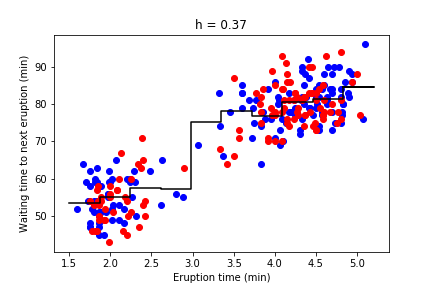
\includegraphics[width=0.6\textwidth]{regressogram.png}
	\end{centering}
\end{figure}
\subsection{Running Mean Smoother}
For the running mean smoother, our prediction function is defined as:
\begin{equation}
\label{rmseq}
\hat{g}(x) = \frac{\sum_{t=1}^Nw(\frac{x-x^t}{h})r^t}{\sum_{t=1}^Nw(\frac{x-x^t}{h})}
\end{equation}
where $h$ is the bin width and our kernel function $w$ is defined as:
\begin{equation}
\label{rmskern}
w(u) = 
	\begin{cases} 
      	1 & \text{if } |u| < 1\\
      	0 & \text{otherwise}
   	\end{cases}
\end{equation}
This function is better in the way that it eliminates the need of an origin parameter. Our results show that the RMSE for Running Mean Smoother is $6.089003211720321$. The plot is given in figure \ref{rmsfig}.
\begin{figure}[ht]
	\centering
	\caption{Running Mean Smoother Plot}
	\label{rmsfig}
	\begin{centering}
		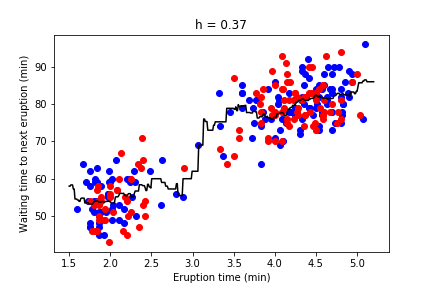
\includegraphics[width=0.6\textwidth]{rms.png}
	\end{centering}
\end{figure}
For our implementation, we reformulated the kernel function. Looking at equations \eqref{rmseq} and \eqref{rmskern}, we see that we have this inequality during our calculations:
\begin{equation}
\left|\frac{x-x^t}{h}\right| < 1
\end{equation}
For $x-x^t > 0$ we can write this as:
\begin{equation}
x-x^t < h
\end{equation}
which yields $x^t > x - h$. For $x - x^t < 0$ we can write this as:
\begin{equation}
x^t-x < h
\end{equation}
which yields $x^t < x + h$. Combining these two inequalities give us:
\begin{equation}
x - h < x^t < x + h
\end{equation}
Note that this seems to double the bin width, so to compensate for that:
\begin{equation}
x - \frac{h}{2} < x^t < x + \frac{h}{2}
\end{equation}
This is how we used it in our implementation. Also, we should note that for any $NaN$ value that occurs we set it to be $0$.
\subsection{Kernel Smoother}
The Kernel Smoother uses a similar prediction function but the kernel function is different. 
\begin{equation}
\hat{g}(x) = \frac{\sum_{t=1}^N K(\frac{x-x^t}{h})r^t}{\sum_{t=1}^N K(\frac{x-x^t}{h})}
\end{equation}
where $h$ is the bin width and our kernel function $K$ is the standart normal distribution function as a Gaussian kernel, which is:
\begin{equation}
K(u) = \frac{1}{\sqrt{2\pi}}e^{-\frac{u^2}{2}}
\end{equation}
Our results show that the RMSE for Running Mean Smoother is $5.874362846844968$. The plot is given in figure \ref{kernelfig}. Also, we should note that for any $NaN$ value that occurs we set it to be $0$.
\begin{figure}[ht]
	\centering
	\caption{Kernel Smoother Plot}
	\label{kernelfig}
	\begin{centering}
		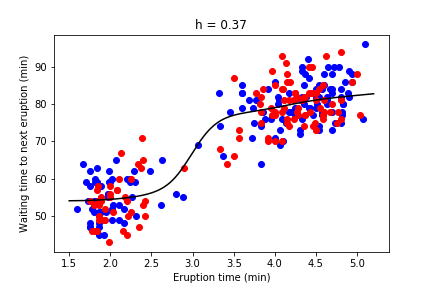
\includegraphics[width=0.6\textwidth]{kernel.png}
	\end{centering}
\end{figure}
Overall, the RMSE is smallest for Kernel Smoother, then Regressogram, and the highest RMSE error is for Running Mean Smoother.
\end{document}